\documentclass[14pt,a4paper]{extreport}
\usepackage[top=2cm, left=3cm, bottom=2cm, right=1cm]{geometry}
\usepackage[utf8x]{inputenc} % Включаем поддержку UTF8
\usepackage[russian]{babel} % Пакет поддержки русского языка
\usepackage{lscape}
\usepackage{fancyhdr}
\usepackage{textcase}
\usepackage{ragged2e}
\usepackage[dvips]{graphicx}
\graphicspath{{/img}}
\parindent=1cm

\title{Курсовой проект}
\author{Михаил Ермолаев}

\begin{document}
%----------ТИТУЛЬНЫЙ-ЛИСТ--------------
	\center
	Министерство образования Республики Беларусь\\
	Учреждение образования «Белорусский государственный университет информатики и радиоэлектроники»
	\vspace*{2cm}
	\endcenter
	\raggedright
	Факультет компьютерных систем и сетей\\
	\medskip
	Кафедра программного обеспечения информационных технологий\\
	\medskip
	Дисциплина:  Базы Данных (БД)
	\vspace*{2cm}
	\center
	ПОЯСНИТЕЛЬНАЯ ЗАПИСКА\\
	к курсовому проекту\\
	на тему\\
	\medskip
	ПС и БД  интернет-ориентированного автоматизированного каталога комплектующих ПК \\
    \medskip
    БГУИР КП 1-40 01 01 507 ПЗ
	\vspace*{4cm}
	\endcenter
	\raggedright
	\hspace*{7.94cm}Студент:  гр. 251005 Ермолаев М.М.\\
	\bigskip
	\hspace*{7.94cm}Руководитель:  Марина И.М.\\
	\center
	\vspace*{7cm}
	Минск 2015
	\pagestyle{empty}
%-------ЛИСТ-ЗАДАНИЯ--------------
	\newpage
	\center
	Учреждение образования\\
	\medskip
	«Белорусский государственный университет информатики и радиоэлектроники»\\
	\medskip
	Факультет компьютерных систем и сетей\\
	\medskip
	\endcenter
	\raggedright
	\hspace*{9.53cm}УТВЕРЖДАЮ\\
	\hspace*{9.53cm}Заведующий кафедрой ПОИТ\\
	\hspace*{9.53cm}\underline{\hspace{6cm}} \\
	\hspace*{11cm}\small (подпись) \normalsize\\
	\hspace*{9.53cm}\underline{\hspace{5cm}}2015 г.\\
	\medskip
	\center
	ЗАДАНИЕ\\
	по курсовому проектированию\\
	\medskip
	\endcenter
	\raggedright
	Студенту \underline{Ермолаеву Михаилу Михайловичу}\\
	\begin{enumerate}
	\item Тема работы \underline{ ПС и БД  интернет-ориентированного автоматизированного каталога комплектующих ПК
 }\\
	\item Срок сдачи студентом законченной работы \underline{09.06.2015}
	\item Исходные данные к работе \underline{Используемый текстовый редактор Sublime text 3. }
	\item Содержание расчётно-пояснительной записки (перечень вопросов, которые подлежат разработке)\\
	\underline{\hspace*{16cm}}\hspace*{-16cm}Введение.\\
    \underline{\hspace*{16cm}}\hspace*{-16cm}1. Обзор аналогов.\\
    \underline{\hspace*{16cm}}\hspace*{-16cm}2. Постановка задачи.\\
	\underline{\hspace*{16cm}}\hspace*{-16cm}3. Разработка программного средства.\\
    \underline{\hspace*{16cm}}\hspace*{-16cm}4. Тестирование программного средства. \\
    \underline{\hspace*{16cm}}\hspace*{-16cm}5. Руководство пользователя. \\
    \underline{\hspace*{16cm}}\hspace*{-16cm}Заключение. \\
	\underline{\hspace*{16cm}}\hspace*{-16cm}Список использованной литературы.\\
    \underline{\hspace*{16cm}}\hspace*{-16cm}Приложение. \\
	\item Перечень графического материала (с точным обозначением обязательных чертежей и графиков)\\
	\underline{1. Схема алгоритма}
	\item Консультант по курсовой работе\\
	\underline{Марина И.М.}
	\item Дата выдачи задания \underline{}
	\item Календарный график работы над проектом на весь период проектирования (с обозначением сроков выполнения и процентом от общего объёма работы):\\
	\underline{\hspace*{16cm}}\hspace*{-16cm}раздел 1 к .. – 15 \% готовности работы;\\
	\underline{\hspace*{16cm}}\hspace*{-16cm}разделы 2, 3 к .. – 30 \% готовности работы;\\
	\underline{\hspace*{16cm}}\hspace*{-16cm}раздел 4 к .. – 60 \% готовности работы;\\
	\underline{\hspace*{16cm}}\hspace*{-16cm}раздел 5, 6 к ..  –  90 \% готовности работы;\\
	\underline{\hspace*{16cm}}\hspace*{-16cm}оформление пояснительной записки и графического материала к\\
	\underline{\hspace*{16cm}}\hspace*{-16cm}.. – 100 \% готовности работы.\\
	\underline{\hspace*{16cm}}\hspace*{-16cm}Защита курсового проекта с 5  по 9 июня 2015 г.\\
	\end{enumerate}
	\hspace*{7cm}РУКОВОДИТЕЛЬ\underline{\hspace*{6cm}}\hspace*{-3.9cm}Марина И.М.\\
	\hspace*{11.5cm}\small (подпись) \normalsize\\
	\bigskip
	Задание принял к исполнению \underline{\hspace*{10.5cm}}\hspace*{-8cm}Ермолаев М.М. ..г.\\
	\hspace*{7cm}\small (дата и подпись студента) \normalsize\\
	%-------СОДЕРЖАНИЕ--------------
	\newpage
	\pagestyle{plain}
	%\renewcommand{\headrulewidth}{0px}
	%\fancypagestyle{plain}{\cfoot{}\rfoot{\thepage}}
	
	\renewcommand\contentsname{\center\normalsize \textbf{СОДЕРЖАНИЕ} \endcenter}
	\tableofcontents
	\endcenter
	%-----ВВЕДЕНИЕ-----
    \justifying
	\newpage
	\addcontentsline{toc}{section}{ВВЕДЕНИЕ}
	\section*{\center\normalsize ВВЕДЕНИЕ \endcenter}
	\par Классификация документов — одна из задач информационного поиска, заключающаяся в отнесении документа к одной из нескольких категорий на основании содержания документа. Классификация может осуществляться полностью вручную, либо автоматически с помощью созданного вручную набора правил, либо автоматически с применением методов машинного обучения. Следует отличать классификацию текстов от кластеризации, в последнем случае тексты также группируются по некоторым критериям, но заранее заданные категории отсутствуют.
    \par Существует три подхода к задаче классификации текстов. Во-первых, классификация не всегда осуществляется с помощью компьютера. Например, в обычной библиотеке тематические рубрики присваиваются книгам вручную библиотекарем. Подобная ручная классификация дорога и неприменима в случаях, когда необходимо классифицировать большое количество документов с высокой скоростью. Другой подход заключается в написании правил, по которым можно отнести текст к той или иной категории. Например, одно из таких правил может выглядеть следующим образом: "если текст содержит слова производная и уравнение, то отнести его к категории математика". Специалист, знакомый с предметной областью и обладающий навыком написания регулярных выражений, может составить ряд правил, которые затем автоматически применяются к поступающим документам для их классификации. Этот подход лучше предыдущего, поскольку процесс классификации автоматизируется и, следовательно, количество обрабатываемых документов практически не ограничено. Более того, построение правил вручную может дать лучшую точность классификации, чем при машинном обучении (см. ниже). Однако создание и поддержание правил в актуальном состоянии (например, если для классификации новостей используется имя действующего президента страны, соответствующее правило нужно время от времени изменять) требует постоянных усилий специалиста. Наконец, третий подход основывается на машинном обучении. В этом подходе набор правил или, более обще, критерий принятия решения текстового классификатора, вычисляется автоматически из обучающих данных (другими словами, производится обучение классификатора). Обучающие данные — это некоторое количество хороших образцов документов из каждого класса. В машинном обучении сохраняется необходимость ручной разметки (термин разметка означает процесс приписывания класса документу). Но разметка является более простой задачей, чем написание правил. Кроме того, разметка может быть произведена в обычном режиме использования системы. Например, в программе электронной почты может существовать возможность помечать письма как спам, тем самым формируя обучающее множество для классификатора — фильтра нежелательных сообщений. Таким образом, классификация текстов, основанная на машинном обучении, является примером обучения с учителем, где в роли учителя выступает человек, задающий набор классов и размечающий обучающее множество.
    \\ \par
    \textbf{Этапы обработки:}
    \begin{enumerate}
      \item  Индексация документов
      \\ \par Построение некоторой числовой модели текста, например в виде многомерного вектора слов и их веса в документе. Уменьшение размерности модели.
      \item  Построение и обучение классификатора
      \\ \par Могут использоваться различные методы машинного обучения: решающие деревья, наивный байесовский классификатор, нейронные сети, метод опорных векторов и др.
      \item  Оценка качества классификации
      \\ \par Можно оценивать по критериям полноты, точности, сравнивать классификаторы по специальным тестовым наборам.[1]
    \end{enumerate}
    \par Для реализации данного приложения был выбран наивный байесовский классификатор в качестве метода машинного обучения. Наивный байесовский классификатор — простой вероятностный классификатор, основанный на применении Теоремы Байеса со строгими (наивными) предположениями о независимости. В зависимости от точной природы вероятностной модели, наивные байесовские классификаторы могут обучаться очень эффективно. Во многих практических приложениях, для оценки параметров для наивных байесовых моделей используют метод максимального правдоподобия; другими словами, можно работать с наивной байесовской моделью, не веря в байесовскую вероятность и не используя байесовские методы. Несмотря на наивный вид и, несомненно, очень упрощенные условия, наивные байесовские классификаторы часто работают намного лучше во многих сложных жизненных ситуациях. Достоинством наивного байесовского классификатора является малое количество данных для обучения, необходимых для оценки параметров, требуемых для классификации.[2]

    %-----Обзор аналагов----
	\newpage
	\addcontentsline{toc}{section}{1 ОБЗОР АНАЛОГОВ}
	\section*{\normalsize\hspace{4ex} 1 ОБЗОР АНАЛОГОВ}
    \par Существует множество классификаторов текста. Наивный байесовский классификатор относится к вероятностным классификаторам. Вероятностные классификаторы рассматривают решение об отнесении документа d к классу c как вероятность P(c|d) принадлежности этого документа к этому классу, и, соответственно, вычисляют её по теореме Байеса.
    \\ \par Данные классификаторы, отличаются простотой в реализации и довольно хорошей скоростью работы, однако не всегда гарантируют точность предположения.
    \\ \par \textbf{Классификаторы на основе решающих правил:}\\
В классификаторах на основе решающих правил, пространство данных моделируется набором правил, на левой стороне которого находится условие на набор признаков, а на правой – метка класса. Набор правил генерируется из обучающей выборки. Для данного тестового объекта мы получаем набор правил, для которых он удовлетворяет их условию на левой стороне. Затем определяем метку класса как функцию от полученных меток класса правил.
    \\ \par \textbf{Метрические алгоритмы классификации:}\\
Одним из простейших способов классифицировать объект является поиск схожего по некоторым параметрам уже классифицированного объекта. Если мера сходства объектов введена достаточно удачно, то, как правило, оказывается, что схожим объектам очень часто соответствуют схожие ответы. В задачах классификации это означает, что классы образуют компактно локализованные подмножества. Это предположение принято называть гипотезой компактности. Для формализации понятия «сходства» вводится функция расстояния в пространстве объектов. Методы обучения, основанные на анализе сходства объектов, называются метрическими, даже если функция расстояния не удовлетворяет всем аксиомам метрики (в частности, аксиоме треугольника).
Примером  метрического классификатора является классификатор Роше. Он легко реализуем и не является ресурсоёмким, однако его качество весьма посредственно.
    \\ \par \textbf{Линейные классификаторы:}\\
    Линейными называют классификаторы, в которых предсказанное значение вычисляется в виде c = w · d + b, где d = (d1, . . . , dl) – нормализованный вектор из частот слов в документе, w – вектор линейных весов той же размерности, что и признаковое пространство, а b – некоторое скалярное значение. Естественной интерпретацией для c в дискретном случае будет разделяющая гиперплоскость между различными классами. Машина опорных векторов (SVM) – один из классификаторов данного вида, который пытается искать «хорошие» линейные разделители между разными классами. Регрессионные модели (такие, как метод наименьших квадратов) – более явные и традиционные статистические методы для классификации текстов. Тем не менее, они обычно используются в случаях, когда целевые переменные являются числовыми, а не номинальными. Наконец, простые нейронные сети также являются одной из форм линейных классификаторов. Самая простая из них, известная как персептрон (или однослойная нейронная сеть) сама по себе создана для линейного разделения и хорошо работает для классификации документов. Тем не менее, используя несколько слоев нейронов, возможно обобщить подход для нелинейного разделения.[3]
\newpage
    \par \small \textbf{1.2 Используемые средства разработки}
    \\ \par Для разработки данного приложения был выбрал язык JavaScript. Данный язык поддерживается всеми современными браузерами, что позволяет приложениям, написанным на этом языке, запускаться на любой платформе. Кроме того, ПО, написанное на JavaScript имеют хорошую производительность.[4]
    \\ \par Для верстки HTML-страницы, будет использоваться HTML,CSS и JavaScript фреймворк - bootstrap, который является открытым и распространяется бесплатно.[1]
    \begin{figure}[h]
    \center{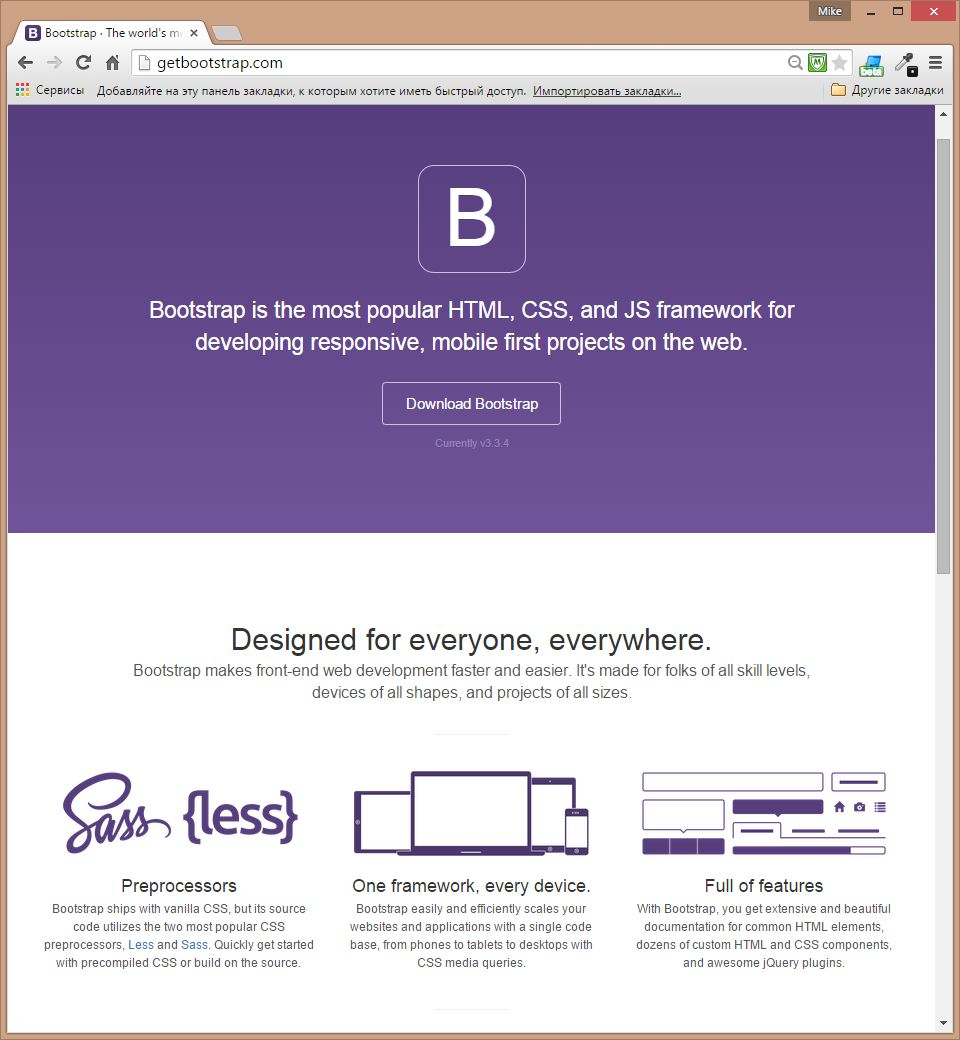
\includegraphics[width=4in,height=4in]{img/bootstrap.jpg}}
    \caption{Сайт фреймворка bootstrap.}
    \label{ris:image}
    \end{figure}
     \newpage
     \par Для отображения результурующего элемента, будет использоваться библиотека React.js, предназначенная для создания элемнтов UI.[5]
    \begin{figure}[h]
    \center{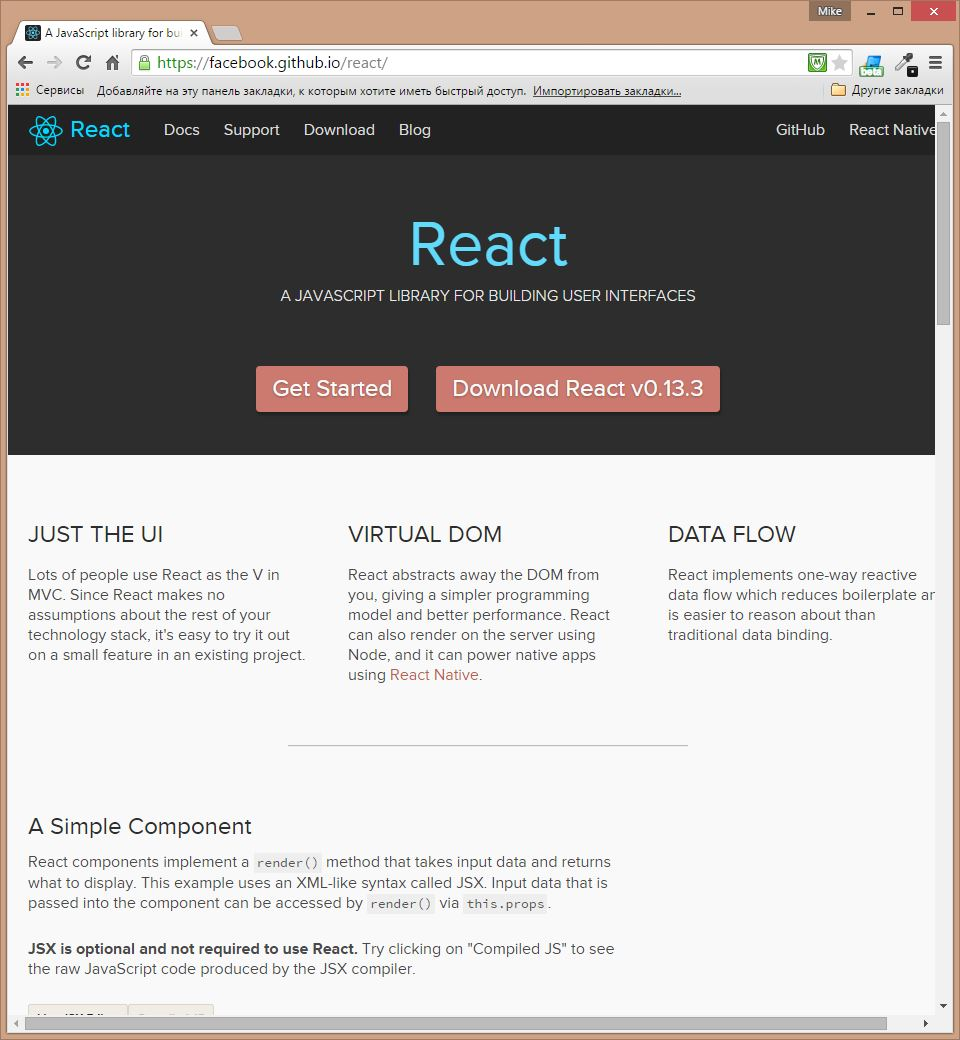
\includegraphics[width=4in,height=4in]{img/react.jpg}}
    \caption{Сайт библиотеки React.js.}
    \label{ris:image}
    \end{figure}
    \newpage
     \par Для написания кода будет использоваться текстовый редактор sublimetext 2. Данное приложение также является бесплатным и очень гибким в настройках, благодоря большому количеству расширений, которые можно установить.
    \begin{figure}[h]
    \center{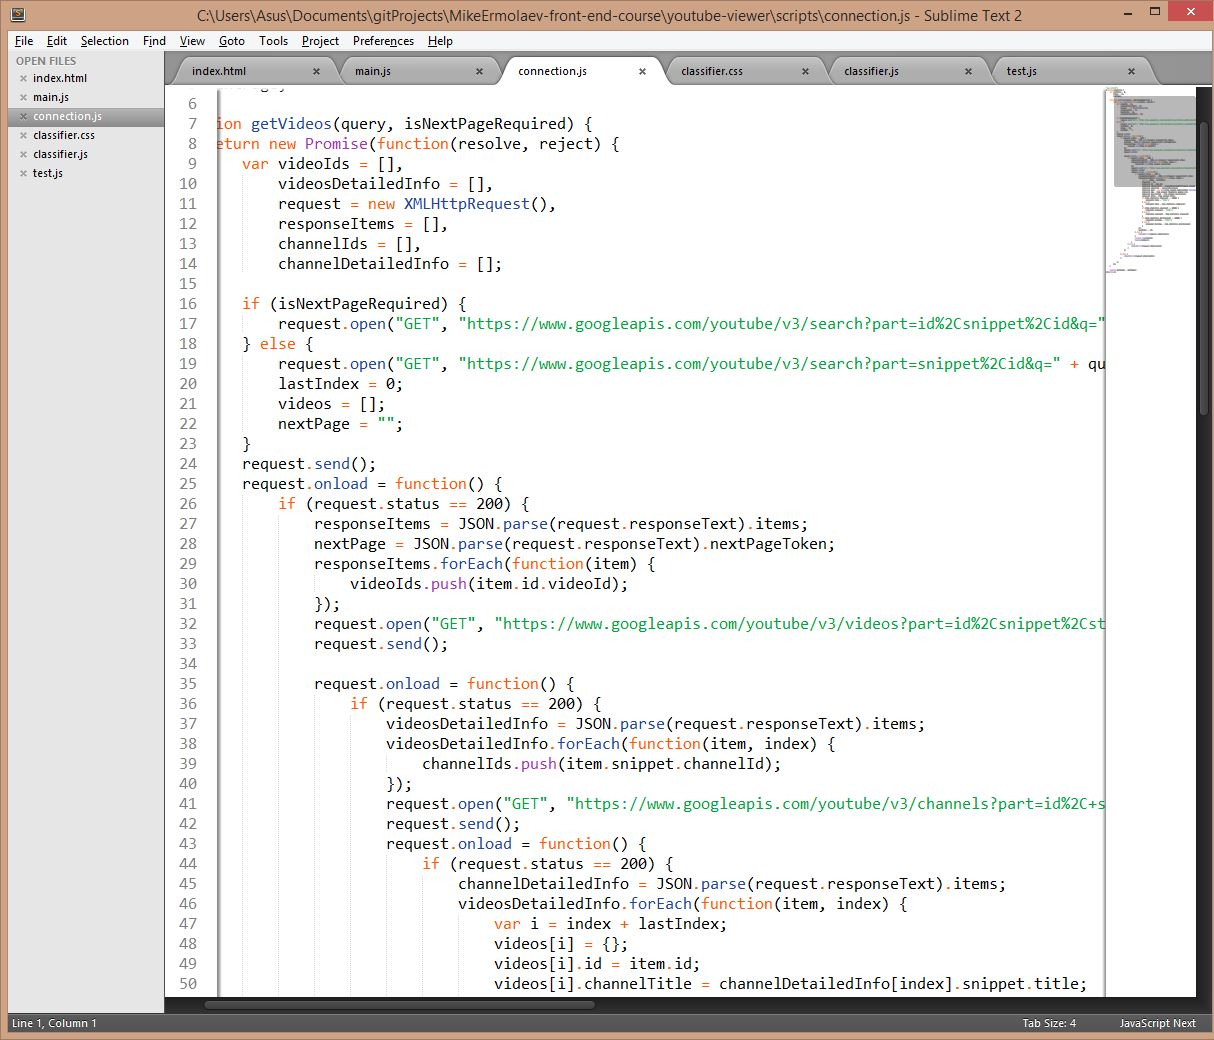
\includegraphics[width=4in,height=4in]{img/sublime.jpg}}
    \caption{Пример импользования sublimetext 2.}
    \label{ris:image}
    \end{figure}
	%-----Постановка задачи----
	\newpage
	\addcontentsline{toc}{section}{2 ПОСТАНОВКА ЗАДАЧИ}
	\section*{\normalsize\hspace{4ex}2 ПОСТАНОВКА ЗАДАЧИ}
	 \par Реализовать веб-приложение, которое выполнять следующие функции:
    \begin{itemize}
      \item Обучение классификатора.
      \item Определение к какому классы относится предоставленный текст.
      \item Установка приложения.
    \end{itemize}
    \par Свойства классификатора:
    \begin{itemize}
      \item Словарь уникальных слов.
      \item Весь набор слов, предоставленных для обучения.
      \item Количество документов, предоставленных для обучения.
    \end{itemize}
    \newpage

	%-----РАЗРАБОТКА ПРИЛОЖЕНИЯ----
	\newpage
	\addcontentsline{toc}{section}{2 РАЗРАБОТКА ПРИЛОЖЕНИЯ}
	\section*{\normalsize\hspace{4ex}2 РАЗРАБОТКА ПРИЛОЖЕНИЯ}
    \par \small \textbf{Функция-конструктор Classifier}
    \\ \par Данная функия инициализирует новый объект классификатора. Конструктор не принимает никаких аргументов. При вызове инициализирует новый объект с пустыми свойствами.
    \begin{figure}[h]
    \center{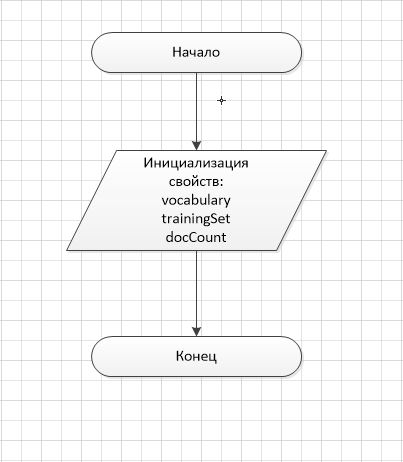
\includegraphics[width=4in,height=6in]{img/construct.jpg}}
    \caption{Блок-схема функции конструктора классификатора}
    \label{ris:image}
    \end{figure}
    \newpage \par \small \textbf{Функция makeBagOfWords}
    \\ \par Данная функция разбивает входную строку на массив слов, пригодный для работы классификатора.
    \begin{figure}[h]
    \center{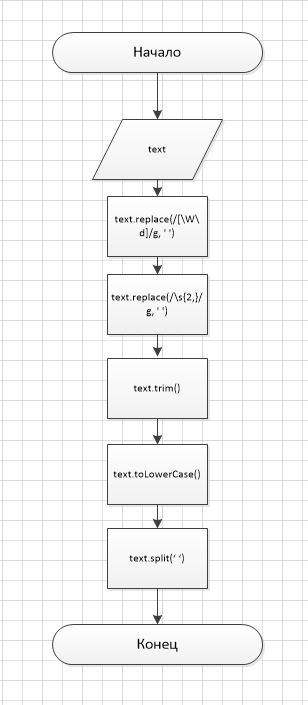
\includegraphics[width=4in,height=6in]{img/bag.jpg}}
    \caption{Блок-схема функции makeBagOfWords}
    \label{ris:image}
    \end{figure}
    \newpage \par \small \textbf{Функция countWordRepetitions}
    \\ \par Данная подсчитывает количество повторяющихся слов в массиве.
    \begin{figure}[h]
    \center{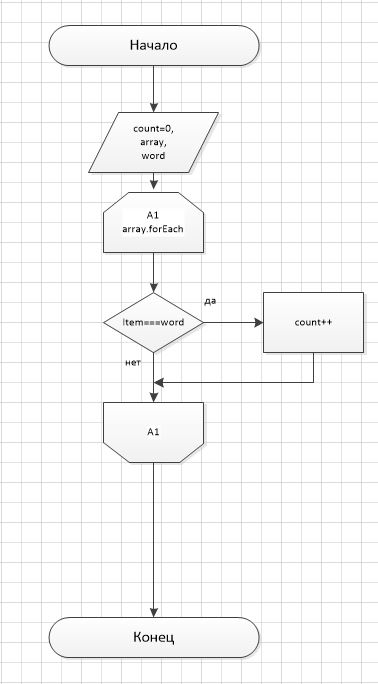
\includegraphics[width=4in,height=6in]{img/count.jpg}}
    \caption{Блок-схема функции countWordRepetitions}
    \label{ris:image}
    \end{figure}
    \newpage \par \small \textbf{Функция Classifier.prototype.train}
    \\ \par Данная функция отвечает за обучение классификатора.
    \par Входные аргументы: group(название класса) и features(текст, принадлежащий данному классу). Если имеются документы, принадлежащие одному классу, то они объединяются в один большой документ. Классу назначается приоритет равный количеству поступивших документов для этого класса. Увеличивается общее количество документов, а также словарь пополняется уникальными словами.
    \\ Ниже представлена блок-схема данной функции.
    \begin{figure}[h]
    \center{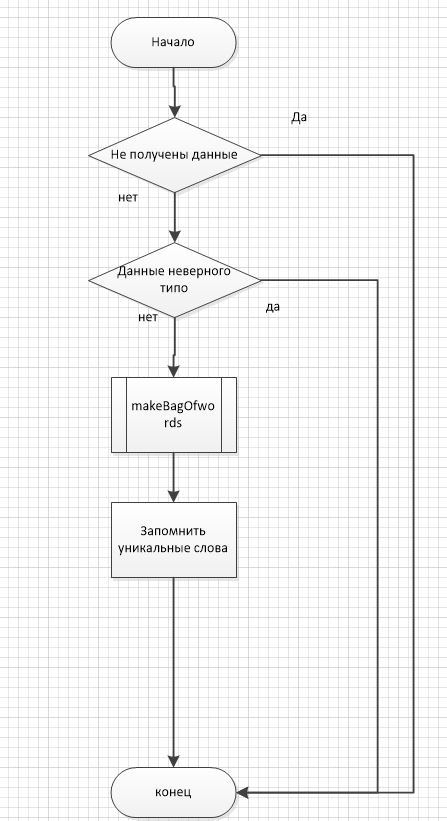
\includegraphics[width=4in,height=6in]{img/train.jpg}}
    \caption{Блок-схема функции Classifier.prototype.train.}
    \label{ris:image}
    \end{figure}
    \newpage \par \textbf{Функция Classifier.prototype.classify}
    \\ \par Данная функция определяет к какому классу принадлежит полученный текст.
     \par Вычисляется общая вероятность принадлежности данного текста к каждому классу, а затем определяется максимальная из них.
    \begin{figure}[h]
    \center{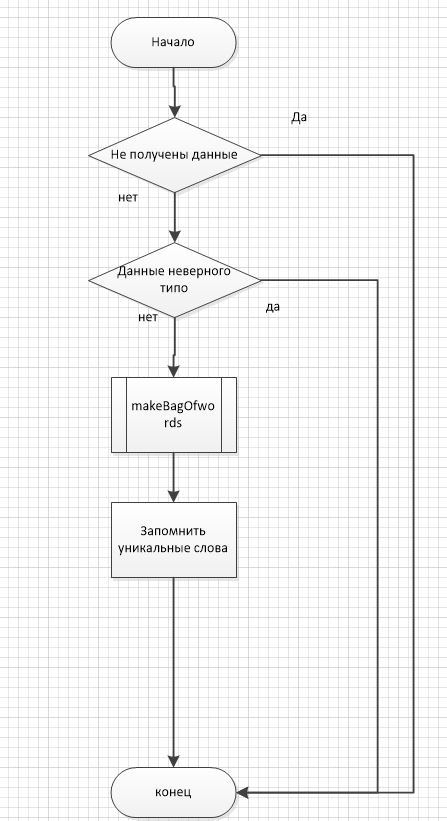
\includegraphics[width=4in,height=6in]{img/classify-block.jpg}}
    \caption{Блок-схема функции Classifier.prototype.classify.}
    \label{ris:image}
    \end{figure}
    \par Для связи с пользователем используется DOM(Document Object Model). Далее описаны методы, которые взаимодействуют с DOM.
    \newpage \par \textbf{Событие отвечающее за обучение классификатора}
    \\ \par Данное событие возникает при нажатии на кнопку Train!.
    \begin{figure}[h]
    \center{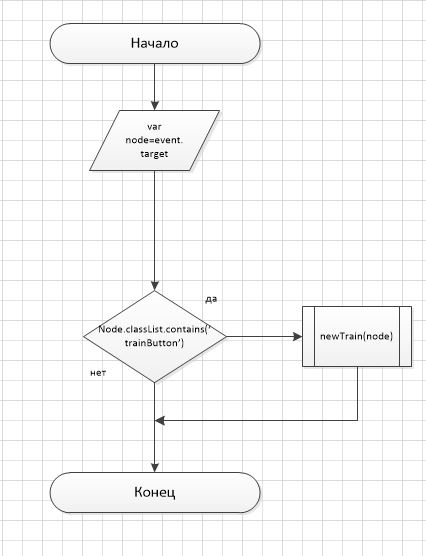
\includegraphics[width=4in,height=6in]{img/trainEvent.jpg}}
    \caption{Блок-схема события нажатия на кнопку Train!}
    \label{ris:image}
    \end{figure}
    \par Событие отлавливается в стадии bubbling и определяется
    \newpage \par \small \textbf{Функция newTrain}
    \\ \par Данная функция отвечает за корректное предоставление данных функции \\ Classifier.prototype.train, а также за отрисовку новых полей для ввода данных.
    \begin{figure}[h]
    \center{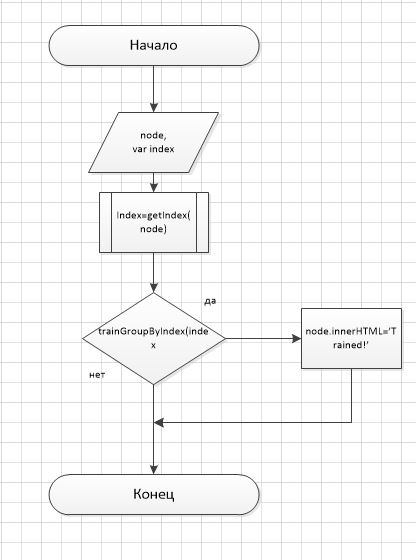
\includegraphics[width=4in,height=6in]{img/newTrain.jpg}}
    \caption{Блок-схема функции newTrain}
    \label{ris:image}
    \end{figure}
    \newpage \par \small \textbf{Функция getIndex}
    \\ \par Данная функция получает индекс текущей строки ввода данных.
    \begin{figure}[h]
    \center{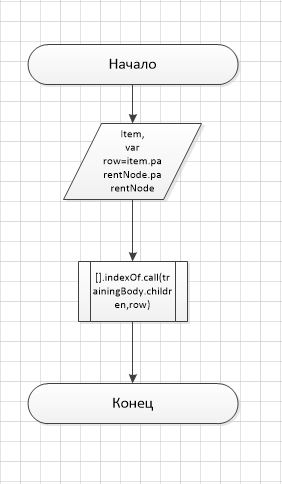
\includegraphics[width=4in,height=6in]{img/getIndex.jpg}}
    \caption{Блок-схема функции newTrain}
    \label{ris:image}
    \end{figure}
    \newpage \par \small \textbf{Функция trainGroupByIndex}
    \\ \par Данная функция обучает классификатор данными, полученными из строки, находящейся по данному индексу.
    \par Ниже представлема блок-схема события trainingBody.onclick.
    \begin{figure}[h]
    \center{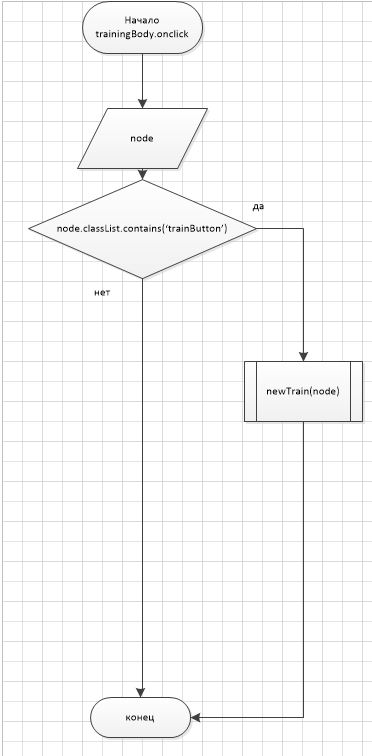
\includegraphics[width=4in,height=6in]{img/event.jpg}}
    \caption{Блок-схема события trainingBody.onclick}
    \label{ris:image}
    \end{figure}
    	%-----ТЕСТИРОВАНИЕ ПРОГРАММНОГО СРЕДСТВА------
    \newpage
    \addcontentsline{toc}{section}{3 ТЕСТИРОВАНИЕ ПРОГРАММНОГО СРЕДСТВА}
    \section*{\normalsize\hspace{4ex}3 ТЕСТИРОВАНИЕ ПРОГРАММНОГО СРЕДСТВА}
    \hspace{18pt} Приложение создавалось в стиле TDD(Test Driven Development)
    \\ \par Данные тесты были написаны при помощи библиотек mocha и chai, которые предназначены для написания тестов на js приложения.
    \begin{figure}[h]
    \center{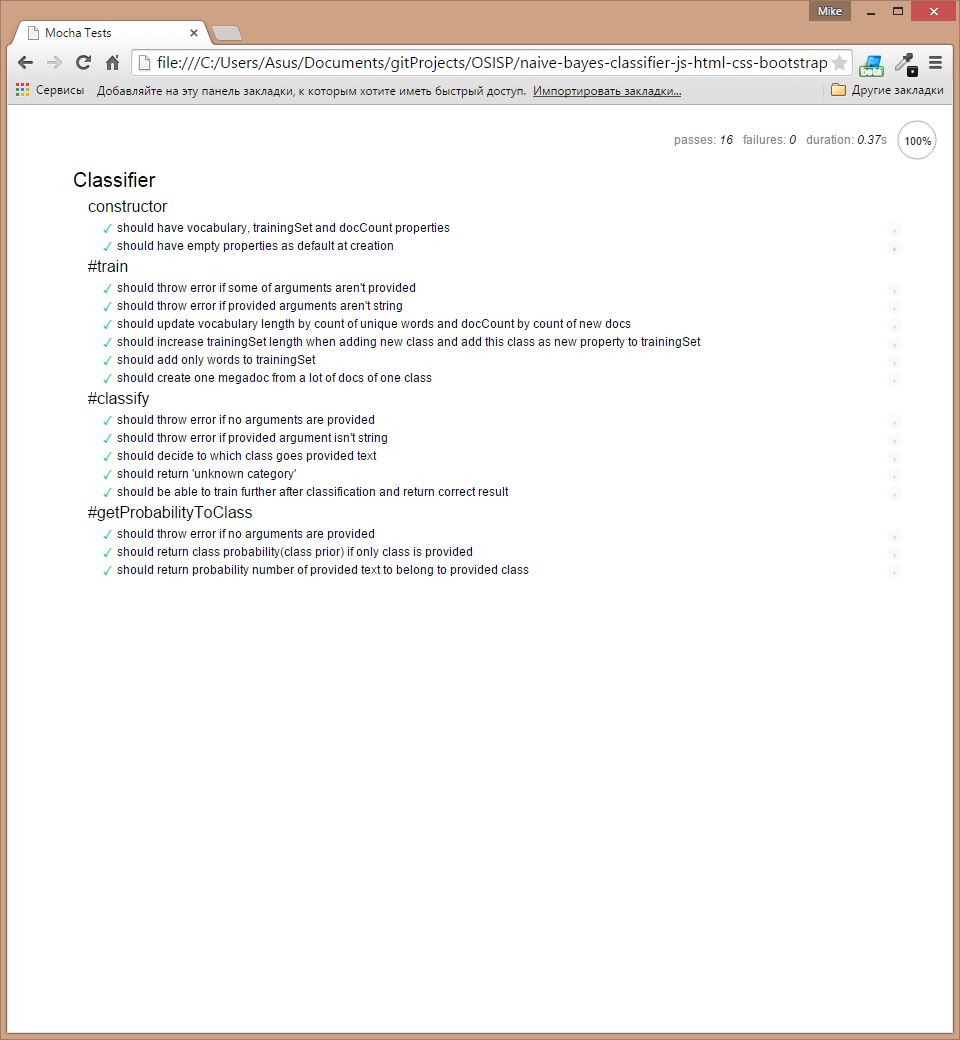
\includegraphics[height=4in]{img/test.jpg}}
    \caption{Скриншот выполнения тестов.}
    \label{ris:image}
    \end{figure}
    \newpage
    \hspace{18pt} \textbf{Тестирование конструктора классификатора}
    \\ \par При создании новый объект классификатора должен:
    \begin{itemize}
      \item  Обладать такими свойствами, как:
                \begin{itemize}
                  \item vocabulary(словарь уникальных слов)
                  \item trainingSet(набор классов и принадлежащих им слов)
                  \item docCount (количество документов, предоставленных для обучения)
                \end{itemize}
      \item Все свойства должны быть по умолчанию пустыми.
    \end{itemize}

    \hspace{18pt} \textbf{Тестирование метода Classifier.prototype.train}
    \\ \par Метод классификатора train должен:
    \begin{itemize}
      \item Сообщить об ошибке, если количество предоставляемых аргументов меньше 2.
      \item Сообщить об ошибке, если предоставляемые аргументы не являются строками.
      \item Обновить значение свойства docCount, в случае необходимости.
      \item Обновить свойство trainingSet.
      \item Добавлять только слова в trainingSet.
      \item В случае добавления новых слов в существующий класс, должен дописать слова в него, а не создавать новый класс в trainingSet
    \end{itemize}

    \hspace{18pt} \textbf{Тестирование метода Classifier.prototype.classify}
    \\ \par Метод классификатора classify должен:
    \begin{itemize}
      \item Сообщить об ошибке, если количество предоставляемых аргументов меньше 1.
      \item Сообщить об ошибке, если предоставляемый аргумент не является строкой.
      \item Отнести к одной из категорий,записанных в свойстве trainingSet.
      \item В случае, если ни одно слово из предоставляемого аргумента не содержится в vocabulary, сообщить о том, что текст принадлежит к неизвестной категории.
      \item Работать корректно при дальнейшем использовании, без повторной инициализации классификатора.
    \end{itemize}

    \hspace{18pt} \textbf{Тестирование метода Classifier.prototype.getProbabilityToClass}
    \\ \par Метод классификатора getProbabilityToClass должен:
    \begin{itemize}
      \item Сообщить об ошибке, если количество предоставляемых аргументов меньше 1.
      \item Вернуть приоритет класса, в случае если предоставлено только название класса.
      \item Вернуть относительную вероятность отнесения предоставляемого текста к предоставляемому классу.
    \end{itemize}
    \newpage
    	%-----РУКОВОДСТВО ПО УСТАНОВКЕ И ИСПОЛЬЗОВАНИЮ ИГРОВОГО ПРИЛОЖЕНИЯ------
	\addcontentsline{toc}{section}{4 РУКОВОДСТВО ПОЛЬЗОВАТЕЛЯ}
	\section*{\normalsize\hspace{4ex}4 РУКОВОДСТВО ПОЛЬЗОВАТЕЛЯ}
	\par\textbf{Установка}
    \\ \par1.Необходимо запустить файл установки.
    \begin{figure}[h]
    \center{
\includegraphics[height=3in]{img/setupstart.jpg}}
    \caption{Запущенный файл установки.}
    \label{ris:image}
    \end{figure}
    \\ \par2.Выбрать путь для установки приложения.
    \begin{figure}[h]
    \center{
\includegraphics[height=3in]{img/setuppath.jpg}}
    \caption{Выбор пути утсановки.}
    \label{ris:image}
    \end{figure}
    \newpage
     \par3.Начать установку.
    \begin{figure}[h]
    \center{
\includegraphics[height=3in]{img/install.jpg}}
    \caption{Завершение подготовки установки.}
    \label{ris:image}
    \end{figure}
    \\
    \par4.Закрыть приложение установки.
    \newpage
    \par\textbf{Приложение}
    \par После того, как приложение было установлено, необходимо зайти в папку с установленным приложением и запустить файл index.html. Откроется браузер со страницей приложения.
    \begin{figure}[h]
    \center{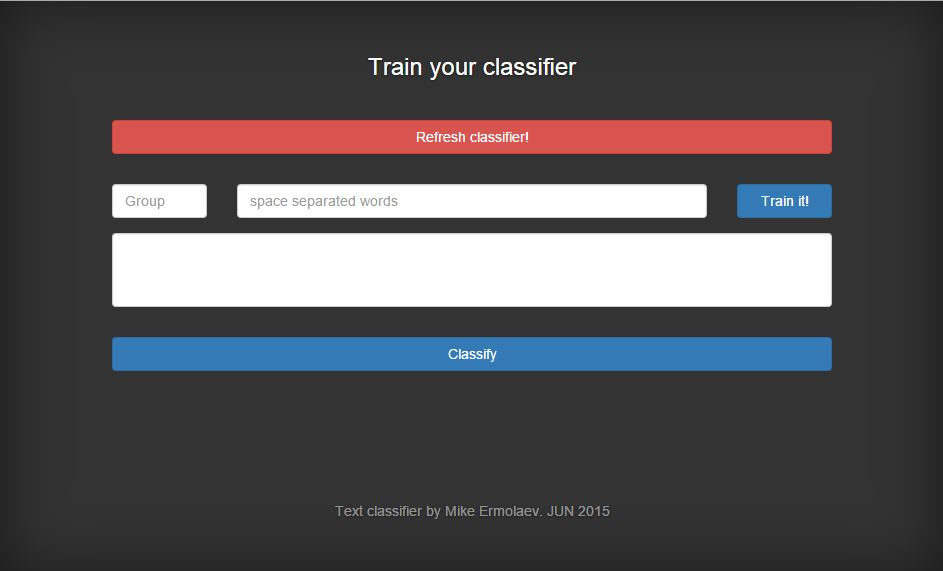
\includegraphics[width=4in,height=3in]{img/app.jpg}}
    \caption{Внешний вид приложения.}
    \label{ris:image}
    \end{figure}
    \par Для обучения классификатора необходимо ввести в соответствующие поля группу и набор слов и нажать на кнопки Train!. В случае, когда поле ввода обучающих данных находится в фокусе, нажатие клавиши Enter будет идентично клику кнопки Train!.
    \begin{figure}[h]
    \center{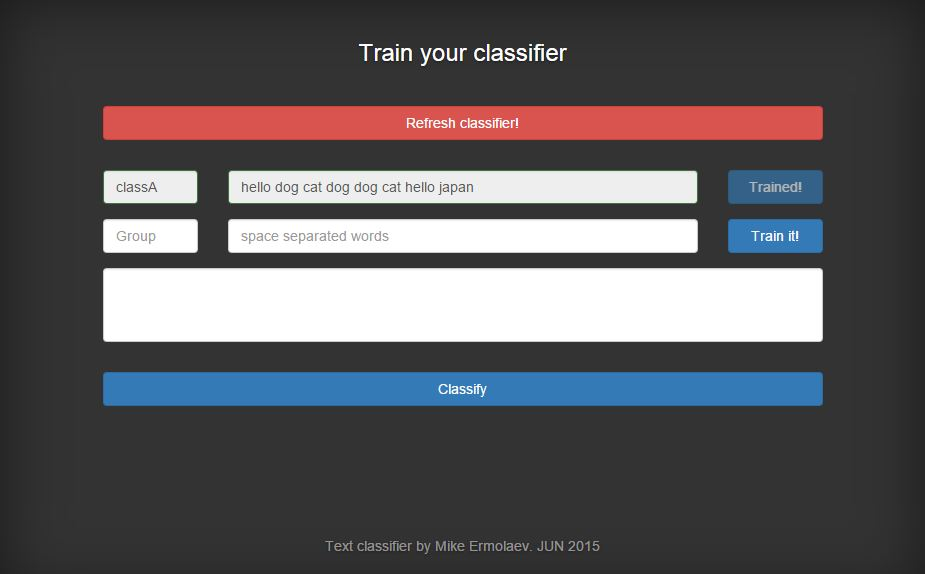
\includegraphics[width=4in,height=3in]{img/nexttrain.jpg}}
    \caption{Обучение классификатора.}
    \label{ris:image}
    \end{figure}
    \newpage
     \par Для классификации текста, нужно ввести его в соответствующее поле и нажать на кнопку Classify.
    \begin{figure}[h]
    \center{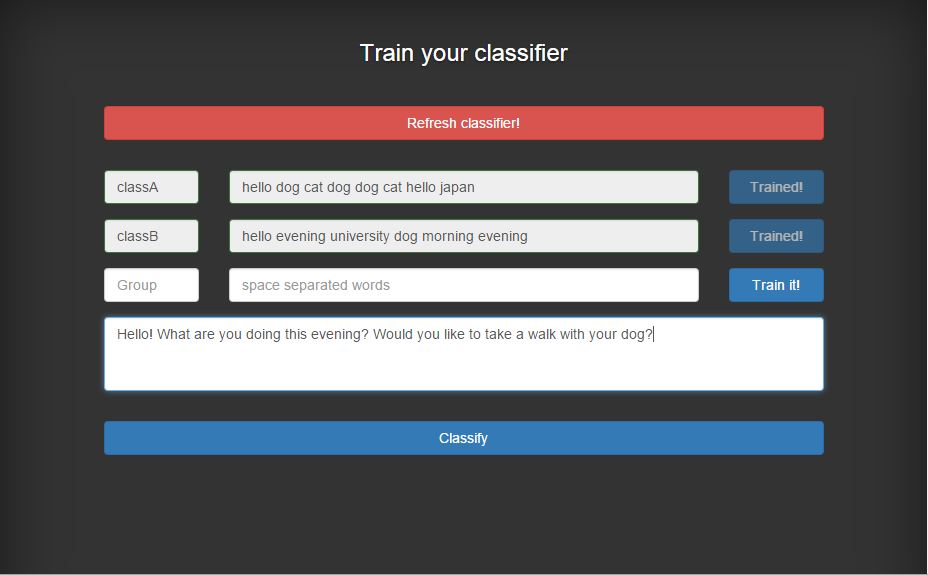
\includegraphics[width=4in,height=3in]{img/classify.jpg}}
    \caption{Подготовка к классификаци.}
    \label{ris:image}
    \end{figure}
    \par Результат представляет собой всплывающее модальное окно,в котором содержится информация о классе и относительной вероятности
    \begin{figure}[h]
    \center{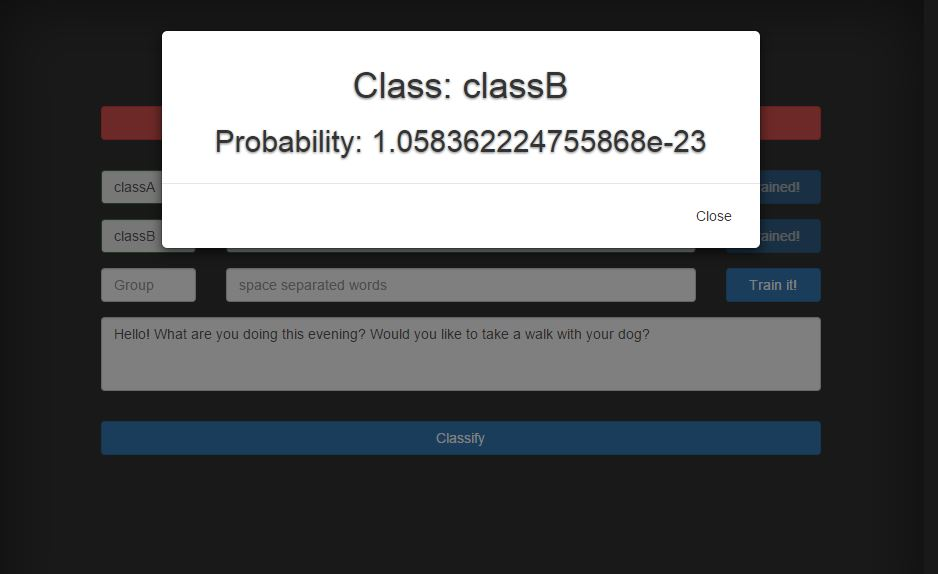
\includegraphics[width=4in,height=3in]{img/result.jpg}}
    \caption{Результат.}
    \label{ris:image}
    \end{figure}
	%-------ЗАКЛЮЧЕНИЕ-------
	\newpage
	\addcontentsline{toc}{section}{ЗАКЛЮЧЕНИЕ}
	\section*{\center\normalsize ЗАКЛЮЧЕНИЕ \endcenter}
	\parВ результате выполнения курсового проекта было разработано приложение Классификатор текста на основе наивного байесовского классификатора.
    \\ \parПроект был выполнен на языке javascript, при помощи библиотеки React.js и bootstrap. Unit-тесты были написаны при помощи библиотек mocha и chai.
    \\ \par В дальнейшем классификатор может быть усовершенствован путем добавления следующих функций:
    \\ \hspace{3ex} 1.Добавление встроенных методов, определяющих принадлежность к конкретному языку.
    \\ \hspace{3ex} 2.Редактирование тренировочного набора.
    \\ \hspace{3ex} 3.Возможность реализации другими алгоритмами.
    \newpage
	%----СПИСОК ИСПОЛЬЗОВАННОЙ ЛИТЕРАТУРЫ-------
	\addcontentsline{toc}{section}{СПИСОК ИСПОЛЬЗОВАННОЙ ЛИТЕРАТУРЫ}
	\section*{\center\normalsize СПИСОК ИСПОЛЬЗОВАННОЙ ЛИТЕРАТУРЫ \endcenter}

    1. ru.wikipedia.org/wiki/Классификация\_документов
    \\2. en.wikipedia.org/wiki/Naive\_Bayes\_classifier
    \\3. http://www.machinelearning.ru/wiki/images/e/ef/NizhibitskyKurs.pdf
    \\4. Дэвид Флэнаган - JavaScript. Подробное руководство, 6-е издание.
    \\5. getbootstrap.com/css/
    \\6. https://facebook.github.io/react/docs/getting-started.html
	%----ПРИЛОЖЕНИЕ Исходный код программы----
	
	\newpage
	\addcontentsline{toc}{section}{ПРИЛОЖЕНИЕ А}
	\section*{\center\normalsize ПРИЛОЖЕНИЕ А\\Исходный код программы \endcenter}
    \par \textbf{Classifier.js}
	\begin{verbatim}

'use strict';

function Classifier() {
	this.vocabulary = [];
	this.trainingSet = {};
	this.docCount = 0;
}
Classifier.prototype.train = function(group, features) {
	var featuresArray,
		that = this;
	if (!group || !features) {
		throw new Error("need some data to work")
	}
	if (typeof group != 'string' || typeof features != 'string') {
		throw new Error('wrong input!');
	}
	featuresArray = makeBagOfWords(features);
	if (Object.keys(that.trainingSet).indexOf(group) > -1) {
		that.trainingSet[group].concat(featuresArray);
		that.trainingSet[group].classPrior++;
	} else {
		that.trainingSet[group] = featuresArray;
		that.trainingSet[group].classPrior = 1;
	}
	that.docCount++;
	featuresArray.forEach(function(feature) {
		if (that.vocabulary.indexOf(feature) == -1) {
			that.vocabulary.push(feature);
		}
	});

};
Classifier.prototype.classify = function(text) {
	var textArray,
		that = this;
	if (!text) {
		throw new Error("need some data to work")
	}
	if (typeof text != 'string') {
		throw new Error('wrong input!');
	}
	textArray = makeBagOfWords(text);
	if (textArray.every(function(word) {
			if (that.vocabulary.indexOf(word) == -1) {
				return true;
			} else {
				return false;
			}
		})) {
		return 'unknown category';
	}
	Object.keys(that.trainingSet).forEach(function(group) {
		that.trainingSet[group].probability = 1;
		textArray.forEach(function(word) {
			that.trainingSet[group].probability *= (countWordRepetitions(word, that.trainingSet[group]) + 1) / (that.trainingSet[group].length + that.vocabulary.length);
		});
		that.trainingSet[group].probability *= that.trainingSet[group].classPrior / that.docCount;
	});
	return Object.keys(that.trainingSet).reduce(function(a, b) {
		if (that.trainingSet[a].probability > that.trainingSet[b].probability) {
			return a;
		} else {
			return b;
		}
	});
};
Classifier.prototype.getProbabilityToClass = function(group, text) {
	var textArray,
		probability=1,
		that=this;
	if(group=='unknown category'){
		return 0;
	}
	if (!text && !group) {
		throw new Error("need some data to work")
	}
	if (!text) {
		if (typeof group != 'string') {
			throw new Error('wrong input!');
		}
		return that.trainingSet[group].classPrior / that.docCount;
	} else {
		if (typeof group != 'string' || typeof text != 'string') {
			throw new Error('wrong input!');
		}
		textArray = makeBagOfWords(text);
		textArray.forEach(function(word){
			probability*=(that.trainingSet[group].classPrior / that.docCount) * ((countWordRepetitions(word, that.trainingSet[group]) + 1) / (that.trainingSet[group].length + that.vocabulary.length));
		});
		return probability;
	}
}

function countWordRepetitions(word, array) {
	var count = 0;
	array.forEach(function(item) {
		if (item === word) {
			count++;
		}
	});
	return count;
}

function makeBagOfWords(text) {
	return text.replace(/[\W\d]/g, ' ').replace(/\s{2,}/g, ' ').trim().toLowerCase().split(' ');
}
    \end{verbatim}
	\par \textbf{main.js}
    \begin{verbatim}
(function(exports) {

	var trainingBody = document.querySelector('.trainingBody'),
		refreshButton = document.querySelector('.refreshButton'),
		classifyButton = document.querySelector('.classifyButton'),
		textarea = document.querySelector('textarea'),
		classifier = new Classifier(),
		template = '\
		<div class="row">\
			<div class="col-xs-2">\
				<input type="text" class="form-control groupName" placeholder="Group">\
			</div>\
			<div class="col-xs-8">\
				<input type="text" class="form-control trainingSet" placeholder="space separated words">\
			</div>\
			<div class="col-xs-2">\
				<button class="btn btn-block btn-primary trainButton">Train it!</button>\
			</div>\
		</div>';

	trainingBody.onkeypress = function(e) {
		if (e.keyCode == 13) {
			var node = e.target;
			newTrain(node);
		}
	}

	trainingBody.addEventListener('click', function(e) {
		var node = e.target;
		if (node.classList.contains('trainButton')) {
			newTrain(node);
		}
	});


	function newTrain(node) {
		var index = getIndex(node);
		if (trainGroupByIndex(index)) {
			node.setAttribute('disabled', null);
			node.innerHTML = "Trained!";
		} else {
			return;
		}
	}

	classifyButton.addEventListener('click', function(e) {
		var res;
		if (textarea.value) {
			textarea.classList.remove('has-error');
			res = classifier.classify(textarea.value);
			reactRender(res, classifier.getProbabilityToClass(res, textarea.value));
		} else {
			e.stopImmediatePropagation();
			textarea.parentNode.classList.add('has-error');
			textarea.focus();
			return false;
		}
	});

	refreshButton.addEventListener('click', function(e) {
		classifier = new Classifier();
		trainingBody.innerHTML = template;
	});

	function getIndex(item) {
		var row = item.parentNode.parentNode;
		return [].indexOf.call(trainingBody.children, row);
	}

	function trainGroupByIndex(index) {
		var groupName = trainingBody.children[index].children[0].children[0],
			trainingSet = trainingBody.children[index].children[1].children[0];

		if (!groupName.value) {
			groupName.parentNode.classList.add('has-error');
			groupName.parentNode.classList.remove('has-success');
			groupName.focus();
			return false;
		} else {
			groupName.parentNode.classList.add('has-success');
			groupName.parentNode.classList.remove('has-error');
		}
		if (!trainingSet.value) {
			trainingSet.parentNode.classList.remove('has-success');
			trainingSet.parentNode.classList.add('has-error');
			trainingSet.focus();
			return false;
		} else {
			trainingSet.parentNode.classList.add('has-success');
			trainingSet.parentNode.classList.remove('has-error');
		}
		classifier.train(groupName.value, trainingSet.value);
		groupName.setAttribute('disabled', '');
		trainingSet.setAttribute('disabled', '');
		trainingBody.insertAdjacentHTML('beforeend', template);
		return true;
	}

})(window)
    \end{verbatim}
	\par \textbf{index.html}
    \begin{verbatim}
<!DOCTYPE html>
<html lang="en">
	<head>
		<meta charset="utf-8">
		<meta http-equiv="X-UA-Compatible" content="IE=edge">
		<meta name="viewport" content="width=device-width, initial-scale=1">
		<title>Text Classifier</title>
		<!-- Bootstrap -->
		<link href="styles/bootstrap.min.css" rel="stylesheet">
		<link href="styles/classifier.css" rel="stylesheet">
		<!--[if lt IE 9]>
		<script src="https://oss.maxcdn.com/html5shiv/3.7.2/html5shiv.min.js"></script>
		<script src="https://oss.maxcdn.com/respond/1.4.2/respond.min.js"></script>
		<![endif]-->
	</head>
	<body>
		<div class="site-wrapper">
			<div class="site-wrapper-inner">
				<div class="cover-container">
					<div class="masthead">
						<h3 class="masthead-brand">Train your classifier</h3>
						<div class="container">
							<button class="btn btn-block btn-danger refreshButton">Refresh classifier!</button>
						</div>
					</div>
					<div class="container trainingBody">
						<div class="row">
							<div class="col-xs-2">
								<input type="text" class="form-control groupName" placeholder="Group">
							</div>
							<div class="col-xs-8">
								<input type="text" class="form-control trainingSet" placeholder="space separated words">
							</div>
							<div class="col-xs-2">
								<button class="btn btn-block btn-primary trainButton">Train it!</button>
								
							</div>
						</div>
					</div>
					<div class="container">
						<textarea class="form-control" rows="3"></textarea>
						<button type="button" data-toggle="modal" data-target="#result" class="btn btn-primary btn-block classifyButton">Classify</button>
						<div class="modal fade" id="result" tabindex="-1" role="dialog" aria-hidden="true">
						</div>
					</div>
					<div class="mastfoot">
						<div class="inner">
							<p>
								Text classifier by Mike Ermolaev. JUN 2015
							</p>
						</div>
					</div>
				</div>
			</div>
		</div>
		<script src="https://code.jquery.com/jquery-2.1.3.min.js"></script>
		<script src="scripts/bootstrap.min.js"></script>
		<script src="https://fb.me/react-0.13.3.js"></script>
		<script src="https://fb.me/JSXTransformer-0.13.3.js"></script>
		<script src="scripts/classifier.js"></script>
		<script type="text/jsx">
		/** @jsx React.DOM **/
			ResultModal = React.createClass({
				render: function() {
					return (
					<div className = "modal-dialog">
							<div className = "modal-content">
											<div className = "modal-body" >
														<h1>Class: {this.props.resultClass}</h1>
														<h2>Probability: {this.props.resultProbability}</h2>
											</div>
											<div className = "modal-footer" >
																	<button type = "button"	className = "btn btn-default" data-dismiss="modal">
															Close
														</button>
											</div>
							</div>
					</div>
					);
				}
			});
			function reactRender(group, prob) {
				React.render( < ResultModal resultClass = {group}
					resultProbability = {prob}/>, document.getElementById('result'));
			}
		</script>
		<script src="scripts/main.js"></script>
	</body>
</html>
    \end{verbatim}
    \newpage
	\addcontentsline{toc}{section}{ПРИЛОЖЕНИЕ Б}
	\section*{\center\normalsize ПРИЛОЖЕНИЕ Б\\Исходный код программы \endcenter}
    \par \textbf{Classifier.js}
	\begin{verbatim}
"use strict";
describe("Classifier", function() {
	var classifier;
	beforeEach(function() {
		classifier = new Classifier();
	});
	describe("constructor", function() {

		it("should have vocabulary, trainingSet and docCount properties", function() {
			expect(classifier).to.have.property('vocabulary');
			expect(classifier).to.have.property('trainingSet');
			expect(classifier).to.have.property('docCount');
			expect(classifier.trainingSet).to.be.an('object')
			expect(classifier.docCount).to.be.equal(0);
		});
		it("should have empty properties as default at creation", function() {
			expect(classifier.vocabulary).to.be.empty;
			expect(classifier.trainingSet).to.be.empty;
			expect(classifier.docCount).to.be.equal(0);
			classifier = new Classifier('asdf', 235425, 'fsdf');
			expect(classifier.vocabulary).to.be.empty;
			expect(classifier.trainingSet).to.be.empty;
			expect(classifier.docCount).to.be.equal(0);
		});
	});
	describe("#train", function() {
		it("should throw error if some of arguments aren't provided", function() {
			expect(function() {
				classifier.train('a');
			}).to.throw("need some data to work");

			expect(function() {
				classifier.train();
			}).to.throw("need some data to work");
		});
		it("should throw error if provided arguments aren't string", function() {
			expect(function() {
				classifier.train(1, {
					asd: 'asd'
				});
			}).to.throw("wrong input!");
		});
		it("should update vocabulary length by count of unique words and docCount by count of new docs", function() {
			expect(classifier.vocabulary).to.have.length(0);
			expect(classifier.docCount).to.be.equal(0);
			classifier.train("spam", "hello buy some viagra");
			expect(classifier.docCount).to.be.equal(1);
			expect(classifier.vocabulary).to.have.length(4);
			expect(classifier.docCount).to.be.equal(1);
			classifier.train("not spam", "hello morning good day");
			expect(classifier.docCount).to.be.equal(2);
			expect(classifier.vocabulary).to.have.length(7);
		});
		it("should increase trainingSet length when adding new class and add this class as new property to trainingSet", function() {
			expect(Object.keys(classifier.trainingSet)).to.have.length(0);
			classifier.train("classA", "qwerty asdf hfd");
			expect(Object.keys(classifier.trainingSet)).to.have.length(1);
			expect(classifier.trainingSet).to.have.property('classA');
			expect(JSON.stringify(classifier.trainingSet.classA)).to.be.equal(JSON.stringify(['qwerty', 'asdf', 'hfd']));
		});
		it("should add only words to trainingSet", function() {
			classifier.train("classA", "qwerty asdf hfd");
			expect(classifier.trainingSet['classA']).to.have.length(3);
			classifier.train("classB", "123 qwerty !@#%,.");
			expect(classifier.trainingSet['classB']).to.have.length(1);
		});
		it("should create one megadoc from a lot of docs of one class", function() {
			classifier.train("classA", "qwerty asdf hfd");
			expect(Object.keys(classifier.trainingSet)).to.have.length(1);
			classifier.train("classA", "tyrt we");
			expect(Object.keys(classifier.trainingSet)).to.have.length(1);
			classifier.train("classA", "gh s");
			expect(Object.keys(classifier.trainingSet)).to.have.length(1);
		});
	});
	describe("#classify", function() {
		var res;
		beforeEach(function() {
			classifier.train("not spam", "hello morning good day");
			classifier.train("spam", "hello buy some viagra");
		});
		it("should throw error if no arguments are provided", function() {
			expect(function() {
				res = classifier.classify();
			}).to.throw("need some data to work");
		});
		it("should throw error if provided argument isn't string", function() {
			expect(function() {
				res = classifier.classify(1);
			}).to.throw("wrong input");
			expect(function() {
				res = classifier.classify({
					lol: "lol"
				});
			}).to.throw("wrong input");
		});
		it("should decide to which class goes provided text", function() {
			res = classifier.classify("good day, i am viagra seller. Do you want to buy some?");
			expect(res).to.be.equal("spam");
		});
		it("should return 'unknown category'", function() {
			res = classifier.classify("unknown words here");
			expect(res).to.be.equal("unknown category");
		});
		it("should be able to train further after classification and return correct result", function() {
			res = classifier.classify("good day, i am viagra seller. Do you want to buy some?");
			expect(res).to.be.equal("spam");
			classifier.train("invitaion", "come at pm evening dinner");
			res = classifier.classify("Good evening! Come to dinner at 6 pm!");
			expect(res).to.be.equal("invitaion");
			classifier.train("spam", "porn porn porn buy drugs");
			res = classifier.classify("Watch porn, eat drugs and buy viagra!");
			expect(res).to.be.equal("spam");
		});
	});
	describe("#getProbabilityToClass", function() {
		var res;
		beforeEach(function() {
			classifier.train("not spam", "hello morning good day");
			classifier.train("spam", "hello buy some viagra");
		});
		it("should throw error if no arguments are provided", function() {
			expect(function() {
				classifier.getProbabilityToClass();
			}).to.throw("need some data to work");
		});
		it("should return class probability(class prior) if only class is provided",function(){
			res = classifier.getProbabilityToClass("spam");
			expect(res).to.be.equal(0.5);
		});
		it("should return probability number of provided text to belong to provided class", function() {
			res = classifier.getProbabilityToClass("spam", "hello good evening buy chips come to me");
			expect(res).to.be.a('number');
		});
	});
});
    \end{verbatim}
\end{document}
